\documentclass[12pt,a4paper]{article}
\usepackage[utf8]{inputenc}
\usepackage[spanish]{babel}
\usepackage{amsmath}
\usepackage{amsfonts}
\usepackage{amssymb}
\usepackage{graphicx}
\usepackage[left=17.3mm,right=17.3mm,top=19mm,bottom=25.4mm]{geometry}
\author{Jose Antonio Andrade Vieyra}
\title{Reporte 2.}
\usepackage{pdfpages}
\usepackage{enumerate}
\usepackage{parskip}
\usepackage{multicol}   
\usepackage{caption}
\captionsetup{font=scriptsize,labelfont=scriptsize}
\usepackage{listings}
\usepackage{color}
\setlength{\parskip}{6pt}
\definecolor{migris}{rgb}{0.5,0.5,0.5}
\definecolor{gray97}{gray}{.97}
\usepackage{subfigure}
\usepackage[subfigure]{tocloft} 
\usepackage{tocloft}
\usepackage{enumerate}
\usepackage{float}
\usepackage{multirow, array}


\setcounter{secnumdepth}{0} 
\setcounter{tocdepth}{1} 
\newcounter{ns}
\addtocounter{ns}{1} 

\lstset{ 
  captionpos=b,                    % Establece la posición de la leyenda del cuadro de código
  frame=single,	                   % Añade un marco al código
  language= Scilab,                 % El lenguaje del código
  numbers=left,                    % Posición de los números de línea (none, left, right).
  numbersep=5pt,                   % Distancia de los números de línea al código
  numberstyle=\small\color{migris}, % Estilo para los números de línea
  backgroundcolor=\color{white},   %color de font
  keywordstyle=\color{blue},       % estilo de las palabras clave
  commentstyle=\color{<green},
  rulecolor=\color{black},         % Si no se activa, el color del marco puede cambiar en los saltos de línea entre textos que sea de otro color, por ejemplo, los comentarios, que están en verde en este ejemplo
  stepnumber=1,                    % Muestra solamente los números de línea que corresponden a cada salto. En este caso: 1,3,5,...
  tabsize=4,                   % Establece el salto de las tabulaciones a 2 espacios
  basicstyle=\scriptsize\ttfamily,  
}
\renewcommand{\lstlistingname}{Código}         %  Listings


\begin{document}

%Inicio portada--------------------------------------------------------------------------------
\begin{titlepage}
\begin{figure}[h!]
\centering

\includegraphics[scale=1]{LOGO.png}
\end{figure}
\hspace{1.3cm}\rule{14.5cm}{3pt} \hspace{-16.5cm}
\rotatebox{270}{\rule{20cm}{3pt}}\hspace{0.43cm} \rotatebox{270}{\rule{18.5cm}{3pt}}\hspace{0.43cm} \rotatebox{270}{\rule{16.98 cm}{3pt}}\vspace{-19cm}
\begin{center}
\hspace{1.3cm} {\bf{\fontsize{20.74pt}{20.74pt} \selectfont INSTITUTO TECNOLÓGICO DE}}\\[0.5cm]
\hspace{1.3cm} {\bf{\fontsize{20.74pt}{20.74pt} \selectfont MORELIA}}\\[2cm]
\hspace{1.3cm} {\fontsize{20.74pt}{20.74pt} \selectfont Control I.}\\[1cm]
\hspace{1.3cm} {\fontsize{20.74pt}{20.74pt} \selectfont Ingeniería Electrónica}\\[1cm]
\hspace{1.3cm} {\bf{\fontsize{17.28pt}{17.28pt} \selectfont Practica \#2:}}\\[0.5cm]
\hspace{1.3cm} {\bf{\fontsize{17.28pt}{17.28pt} \selectfont Poles and Zeros found by inspection.}}\\[1.5cm]
\hspace{1.3cm} {\fontsize{17.28pt}{17.28pt} \selectfont Presentan:}\\[0.8cm]
\hspace{1.3cm} {\bf{\fontsize{14pt}{14pt} \selectfont José Antonio Andrade Vieyra No. Control:14121110}}\\[0.5cm]
\hspace{1.3cm} {\bf{\fontsize{14pt}{14pt} \selectfont Gerardo Garcia Torres No. Control: 14121118}}\\[1cm]
\hspace{1.3cm} {\fontsize{17.28pt}{17.28pt} \selectfont Maestro:}\\[0.5cm]
\hspace{1.3cm} {\bf{\fontsize{14pt}{14pt} \selectfont Gerardo Marx Chávez Campos}}
\end{center}   
\vspace{1.8cm}\hspace{1.3cm}\raggedleft {\fontsize{11pt}{11pt} \selectfont Morelia, Michoacán 24 de Noviembre del 2017}
\end{titlepage}
%Final portada---------------------------------------------------------------------------------

%Introducción-------------------------------------------------------------------------------
\newpage
\section{Introducción.}
La manera de encontrar los polos y las raíces se pueden encontrar mediante la función de transferencia, estos se identifican con la factorización de la función de transferencia y de esta manera encontrarlos de una manera sencilla. El proceso de encontrar la función de transferencia y desarrollarla es una proceso complicado y laborioso.\\[12pt]
En este reporte se muestra la forma de obtener la función de transferencia de dos formas, el método de inspección y el método algebraico. Como se puede observar, el método de inspección es la manera fácil y rápida de encontrar la función de transferencia, por lo tanto se obtienen los polos y raíces mientras que con el método algebraico es el proceso  más largo y tedioso para obtenerlos como se mostrara en las próximas páginas.\\[12pt]
Se utilizó un circuito de primer orden usando 3 resistencias y un inductor. Dado este sistema se encontró la función de transferencia con los dos métodos dichos, aparte se hizo la simulación de esté y finalmente se hicieron mediciones en el laboratorio.\\[12pt]
Considerando el sistema descrito por la Ecuación \ref{Ecuacion1} dada tomando la transformada de Laplace y resolviendo para la razón de salida $Y(s)$ y a la entrada $X(s)$, la función de transferencia del sistema $H(s)$ será:\\
\begin{equation}
\centering
H(s) = \dfrac{Y(s)}{X(s)} = \dfrac{a_{m}s^{m}+a_{m-1}s^{m-1}+.......+a_{0}}{b_{m}s^{m}+b_{m-1}s^{m-1}+.......+b_{0}}
\label{Ecuacion1}
\end{equation}\\
Las raíces del denominador son denominadas los polos de la función de transferencia. Las raíces del numerador son denominados los ceros de la función de transferencia (estos valores de s hacen a la función de transferencia igual a cero). Factorizando la Ecuación \ref{Ecuacion1} da como resultado la Ecuación \ref{Ecuacion2}:\\
\begin{equation}
\centering
H(s) = \left(\dfrac{a_{0}}{b_{0}}\right)\left(\dfrac{(1+....+\frac{a_{m-1}}{a_{0}}s^{m-1} + \frac{a_{m}}{a_{0}}s^{m})}{(1+....+\frac{b_{m-1}}{b_{0}}s^{m-1} + \frac{b_{m}}{b_{0}}s^{m})}\right) = G_{0}\left(\dfrac{(1+\frac{s}{\omega_{z1}})(1+\frac{s}{\omega_{z2}})....}{(1+\frac{s}{\omega_{p1}})(1+\frac{s}{\omega_{p2}})....}\right)
\label{Ecuacion2}
\end{equation}\\
Donde $W_{zi}$ son los ceros y $W_{pi}$ son los polos.
%------------------------------------------------------------------------------------------

%Desarrollo-------------------------------------------------------------------------------
\section{Metodología.}
El circuito usado para esta practica es el que se muestra en la Figura \ref{Figura1}:\\
\begin{figure}[h!]
\centering
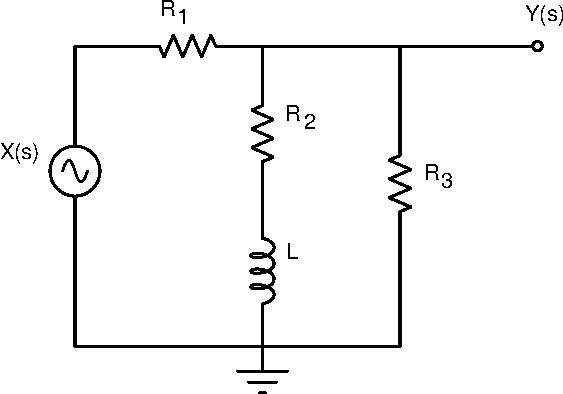
\includegraphics[scale=0.7]{Circuito.pdf}
\caption{Circuito usado para la práctica.}
\label{Figura1}
\end{figure}

\newpage
Dado el sistema anterior para la primera parte se tuvo que obtener la función de transferencia con los dos métodos, con el de inspección y el algebraico. Posteriormente, se tuvo que usar la función hecha en Scilab en la práctica 1 para obtener la respuesta de la función.
\subsection{Función de transferencia con el método de inspección.}
Primero se tiene que hacer el análisis del sistema cuando $s = 0$, es decir, en CD, con esto se puede obtener $G_{0}$, ya que es un inductor, cuando hay corriente directa se hace corto, entonces nuestro voltaje de salida es:\\
\begin{center}
$V_{o} = V_{i}\left(\dfrac{R_{2}||R_{3}}{R_{2}||R_{3}+R_{1}}\right)$
\end{center}
Entonces la ganancia en CD ($G_{0}$) es:\\
\begin{center}
$G_{0}=\dfrac{R_{2}||R_{3}}{R_{2}||R_{3}+R_{1}}$
\end{center}
Ahora hay que obtener el cero de la función de transferencia, esto es cuando es cero en el voltaje de salida. La manera para que $V_{o}$ sea igual a cero es que se forme un corto en $R_{2}$ y $L$, esto pasaría a una cierta frecuencia, entonces:\\
\begin{center}
$R_{2} + Z_{L} = 0$ como $Z_{L} = j\omega L = sL$\\[12pt]
$R_{2} + sL = 0$\\[12pt]
$s = \dfrac{-R_{2}}{L}$\\[12pt]
$\omega_{z1} = \dfrac{R_{2}}{L}$
\end{center}
Solo falta calcular el polo para el sistema de primer orden, este se calcula fácilmente con el inverso de la constante del tiempo del inductor $\tau$.\\
\begin{center}
$\tau = \dfrac{L}{R_{eq}}$
\end{center}
Para obtener la equivalencia de resistencia, se pone en corto la fuente de voltaje y la resistencia equivalente seria en las terminales del inductor, entonces:\\
\begin{center}
$R_{eq}=R_{2} + R_{1}||R_{3}$
\end{center}
Por lo tanto, el polo es:
\begin{center}
$\omega_{p1} = \dfrac{1}{\tau} = \dfrac{1}{\frac{L}{R_{eq}}} = \dfrac{R_{eq}}{L} = \dfrac{R_{2} + R_{1}||R_{3}}{L}$
\end{center}
Entonces nuestra función de transferencia de primer orden es:
\begin{center}
$H(s)=  G_{0}\left(\dfrac{(1+\frac{s}{\omega_{z1}})}{(1+\frac{s}{\omega_{p1}})}\right)= \left(\dfrac{R_{2}||R_{3}}{R_{2}||R_{3}+R_{1}}\right)\left(\dfrac{(1+\frac{sL}{R_{2}})}{(1+\frac{sL}{R_{2} + R_{1}||R_{3}})}\right)$
\end{center}

\newpage
\subsection{Función de transferencia con el método algebraico.}
Para obtener la función de transferencia con este método es obteniendo la relación de voltaje de salida entre el voltaje de entrada de la Figura \ref{Figura1} y esto se hace con un divisor de tensión, primero obtenemos el paralelo de las resistencias siguientes:\\
\begin{center}
$Z_{L} = sL$\\[12pt]
$Z_{int} = sL + R_{2}$\\[12pt]
$Z_{int}||R_{3}= \dfrac{R_{3}(sL + R_{2})}{R_{3}+sL+R_{2}}$
\end{center}
Ya obteniendo la equivalencia de resistencias y la impedancia del inductor se simplifica más el divisor de tensión que se muestra a continuación:\\
\begin{center}
$V_{out}=V_{in}\left(\dfrac{Z_{int}||R_{3}}{Z_{int}||R_{3} + R_{1}}\right)$
\end{center}
Se obtiene la relación $\frac{V_{out}}{V_{in}}$ que es $H(s)$ y se desarrolla para obtener la función de transferencia, todo el desarrollo y simplificación se muestra a continuación:\\
\begin{center}
$H(s)= \left(\dfrac{Z_{int}||R_{3}}{Z_{int}||R_{3} + R_{1}}\right) = \left(\dfrac{\frac{R_{3}(sL + R_{2})}{R_{3}+sL+R_{2}}}{\frac{R_{3}(sL + R_{2})}{R_{3}+sL+R_{2}} + R_{1}}\right) = \dfrac{R_{3}(sL+R_{2})}{R_{3}(sL + R_{2}) + R_{1}(R_{3}+sL+R_{2})}$\\[12pt]
$=\dfrac{R_{2}R_{3}(1+\frac{sL}{R_{2}})}{sLR_{3} + sLR_{1} + R_{2}R_{3} + R_{1}R_{3}+R_{1}R_{2}}=\dfrac{R_{2}R_{3}(1+\frac{sL}{R_{2}})}{sL(R_{1}+R_{3}) + R_{2}R_{3} + R_{1}(R_{2}+R_{3})}$\\[12pt]
$=\dfrac{R_{2}R_{3}(1+\frac{sL}{R_{2}})}{sL(R_{1}+R_{3}) + R_{2}R_{3} + R_{1}(R_{2}+R_{3})}\left(\dfrac{\frac{1}{R_{2} + R_{3}}}{\frac{1}{R_{2} + R_{3}}}\right)=\dfrac{\frac{R_{2}R_{3}}{R_{2}+R_{3}}(1+\frac{sL}{R_{2}})}{sL(\frac{R_{1} +R_{3}}{R_{2}+R_{3}})+ \frac{R_{2}R_{3}}{R_{2} + R_{3}} + R_{1}}$\\[12pt]
Como $R_{2}||R_{3} = \dfrac{R_{2}R_{3}}{R_{2}+R_{3}}$\\[12pt]
$=\dfrac{R_{2}||R_{3}(1+\frac{sL}{R_{2}})}{(R_{2}||R_{3}+R_{1})(1+\frac{sL(R_{1}+R_{3})}{(R_{2}+R_{3})(R_{2}||R_{3}+R_{1})})}=\left(\dfrac{R_{2}||R_{3}}{R_{2}||R_{3}+R_{1}}\right)\left(\dfrac{(1+\frac{sL}{R_{2}})}{1+\frac{sL(R_{1}+R_{3})}{R_{2}R_{3}+R_{1}(R_{2}+R_{3})}}\right)$\\[12pt]
$=\left(\dfrac{R_{2}||R_{3}}{R_{2}||R_{3}+R_{1}}\right)\left(\dfrac{(1+\frac{sL}{R_{2}})}{1+\frac{sL(R_{1}+R_{3})}{R_{2}R_{3}+R_{1}R_{2}+R_{1}R_{3}}}\right)=\left(\dfrac{R_{2}||R_{3}}{R_{2}||R_{3}+R_{1}}\right)\left(\dfrac{(1+\frac{sL}{R_{2}})}{1+\frac{sL(R_{1}+R_{3})}{R_{2}(R_{1}+R_{3})+R_{1}R_{3}}}\right)$\\[12pt]
$=\left(\dfrac{R_{2}||R_{3}}{R_{2}||R_{3}+R_{1}}\right)\left(\dfrac{(1+\frac{sL}{R_{2}})}{1+\frac{sL(R_{1}+R_{3})}{(R_{1}+R_{3})(R_{2}+\frac{R_{1}R_{3}}{R_{1}+R_{3}})}}\right)=\left(\dfrac{R_{2}||R_{3}}{R_{2}||R_{3}+R_{1}}\right)\left(\dfrac{(1+\frac{sL}{R_{2}})}{1+\frac{sL}{R_{2}+R_{1}||R_{3}}}\right)$\\[12pt]
Entonces nuestro resultado obtenido con este método es:\\
\begin{center}
$H(s)=\left(\dfrac{R_{2}||R_{3}}{R_{2}||R_{3}+R_{1}}\right)\left(\dfrac{(1+\frac{sL}{R_{2}})}{(1+\frac{sL}{R_{2}+R_{1}||R_{3}})}\right)$
\end{center}
\end{center}
%-----------------------------------------------------------------------------------------

%Resultados y discuciones-----------------------------------------------------------------
\section{Resultados y discusiones.}
En esta parte se tuvo que usar Scilab y LTspice, Scilab para ver la respuesta de la función de transferencia y LTspice para simular el circuito y obtener la señal de salida en el tiempo y ver la respuesta en frecuencia de la salida (Diagrama de bode). Al final de esta sección se pondrán también los resultados obtenidos de las mediciones realizadas en el laboratorio.\\[12pt]
Para nuestro circuito se propuso los siguientes valores de resistencias y del inductor:\\
\begin{center}
$R_{1}=1.2k\Omega$, $R_{2}=1.2k\Omega$, $R_{3}=15k\Omega$ y $L=4.2mH$
\end{center}
Con esto nuestra función de transferencia queda así y se muestra en la Ecuación \ref{Ecuacion3}\\
\begin{center}
$H(s)=\left(\dfrac{R_{2}||R_{3}}{R_{2}||R_{3}+R_{1}}\right)\left(\dfrac{(1+\frac{sL}{R_{2}})}{(1+\frac{sL}{R_{2}+R_{1}||R_{3}})}\right)$\\[12pt]
$H(s)=\left(\dfrac{(1.2k\Omega)||(15k\Omega)}{(1.2k\Omega)||(15k\Omega)+(1.2k\Omega)}\right)\left(\dfrac{(1+\frac{(4.2mH)s}{1.2k\Omega})}{(1+\frac{(4.2mH)s}{1.2k\Omega+(1.2k\Omega)||(15k\Omega)})}\right)$\\[12pt]
$H(s)=\left(0.481)\right)\left(\dfrac{(1+(3.5x10^{-6})s)}{(1+(1.82x10^{-6})s)}\right)$
\end{center}
\begin{equation}
\centering
H(s)=\dfrac{(1.684x10^{-6})s+0.481}{(1.82x10^{-6})s+1}
\label{Ecuacion3}
\end{equation}
\subsection{Respuesta de la función de transferencia en Scilab.}
Para obtener la respuesta de la función de transferencia en Scilab, se tiene la siguiente forma de coeficientes:
\begin{center}
$H(s)=\dfrac{bs+c}{ds+a}$
\end{center}
Entonces dada la Ecuación \ref{Ecuacion3} nuestros coeficientes a ingresar en la función son los siguientes:\\
\begin{center}
$a = 1$, $b = 1.684x10^{-6}$, $c = 0.481$ y $d=1.82x10^{-6}$  
\end{center}
El código que se uso para obtener la respuesta es el que se muestra en el Código 1:\\
\begin{center}
\lstinputlisting[caption=Código hecho por nosotros para obtener respuesta de escalón unitario.]{obtenertrans.sce}
\end{center}
Entonces los datos a ingresar en la función son los anteriores y el tiempo que se puso fue de 0.5ms porque la frecuencia que se estuvo trabajando fue de 2kHz. A continuación se muestra la gráfica obtenida en Scilab. Se agrego el comando xgrid(2) para que se pusieran las divisiones en la gráfica.
\newpage
\begin{figure}[h!]
\centering
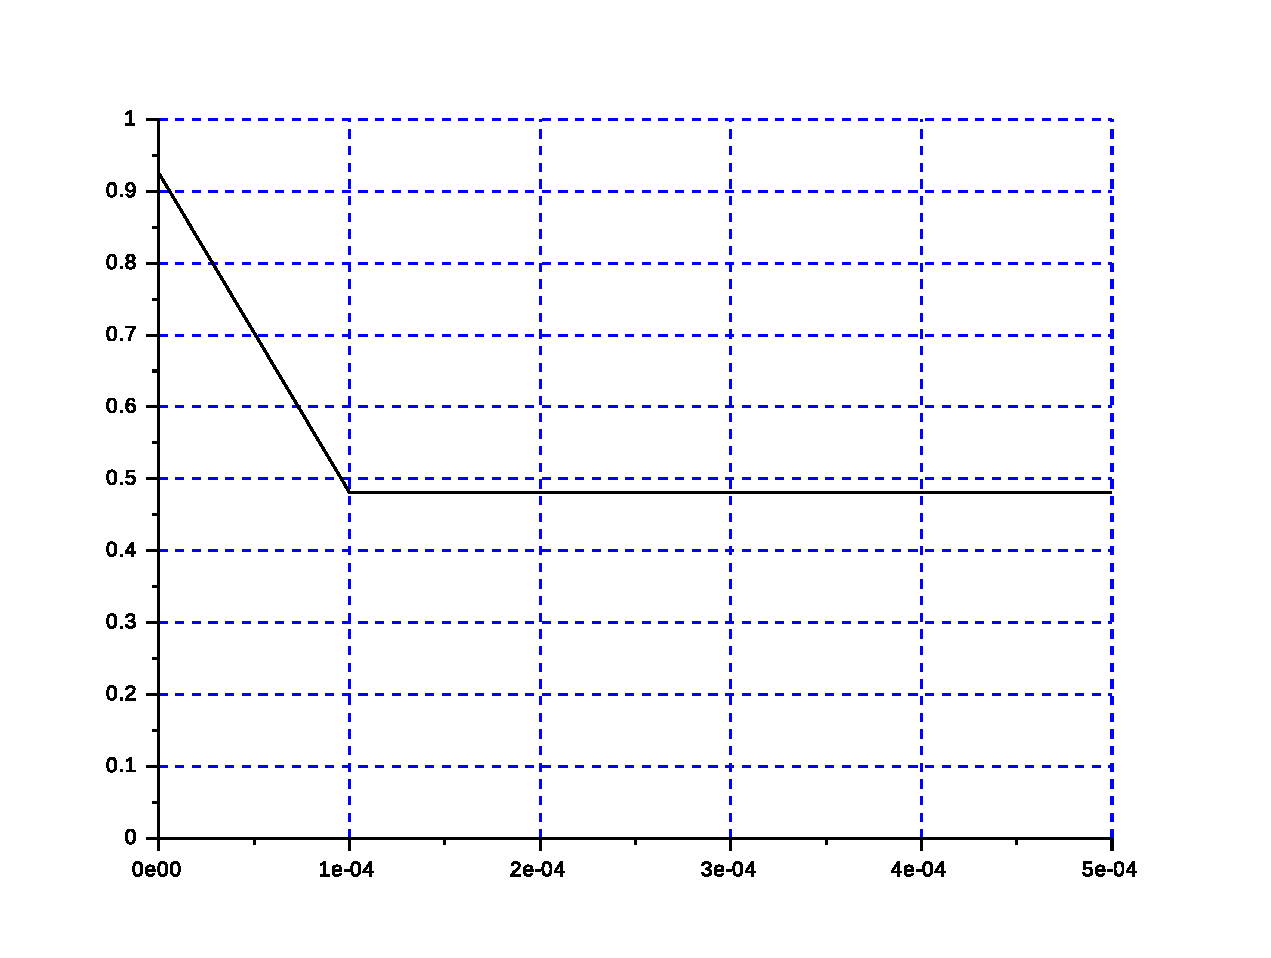
\includegraphics[scale=0.5]{Grafica.pdf}
\caption{Gráfica de respuesta con 500us de tiempo.}
\label{Figura2}
\end{figure}
Se puede observar la descarga del inductor, por lo que la respuesta obtenida en Scilab es correcta y se concluye que la función de transferencia obtenida es la correcta.
\subsection{Simulación en LTspice.}
En este apartado se simuló el circuito en LTspice, fueron dos simulaciones, una en el tiempo y la otra respecto a la frecuencia. A continuación se muestran los dos códigos que se usaron.
\begin{center}
\lstinputlisting[caption=Código para simulación en el tiempo.]{Draft1.cir}
\end{center}
\begin{center}
\lstinputlisting[caption=Código para simulación en la frecuencia.]{Draft2.cir}
\end{center}
Se puede observar que en el primer código es el transitorio y que se usa una señal de pulso cuadrada con 5V de amplitud y con un periodo de 500us siendo su frecuencia de 2kHz.\\[12pt]
En el segundo código se puede observar que se usa el barrido en frecuencia con una señal de 1Vpp y se hace el barrido desde 10Hz hasta 500KHz en decadas de 10.\\[12pt]
A continuación se muestran la salida de voltaje en ambas simulaciones en las Figura \ref{Figura3} y \ref{Figura4} respectivamente.
\newpage
\begin{figure}[h!]
\centering
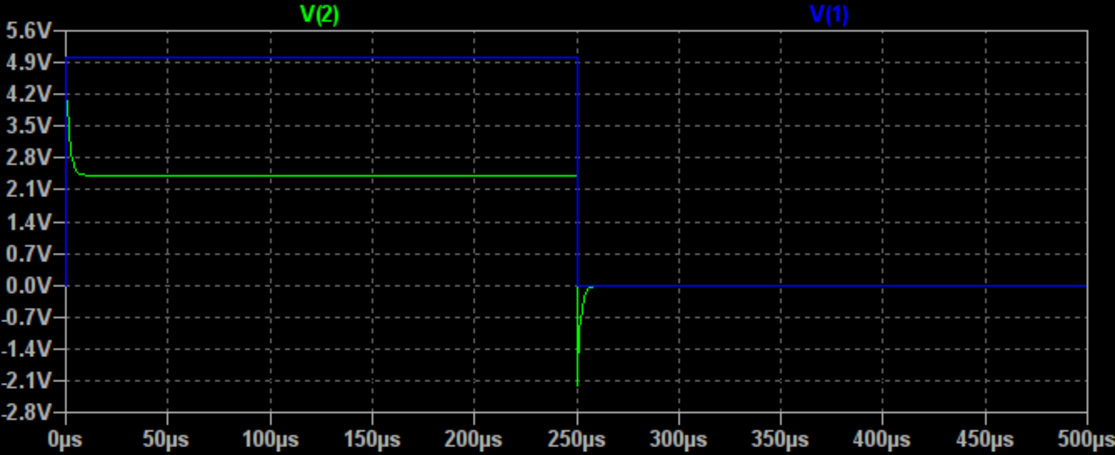
\includegraphics[scale=0.8]{Simulacion_transitoria.pdf}
\caption{Señal de salida en el tiempo.}
\label{Figura3}
\end{figure}
\begin{figure}[h!]
\centering
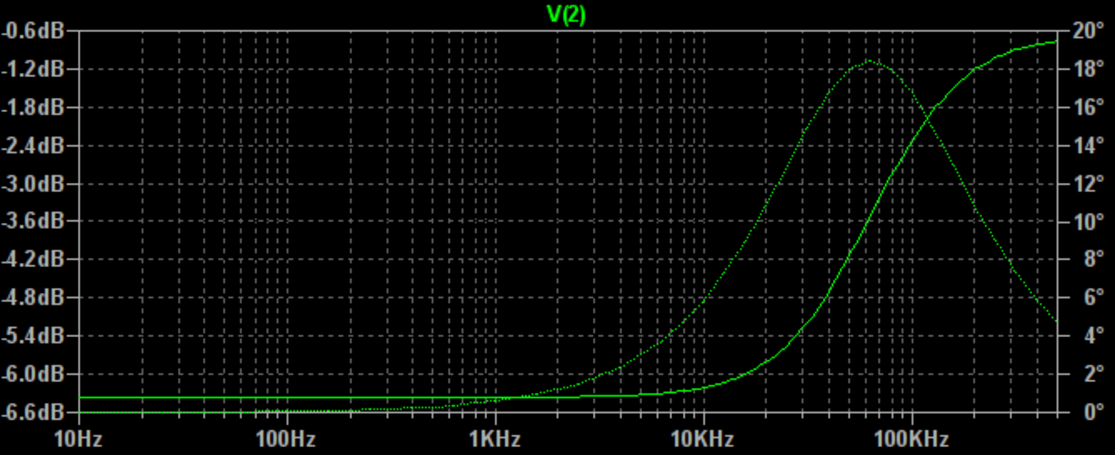
\includegraphics[scale=0.8]{Simulacion_frecuencia.pdf}
\caption{Señal de salida en la frecuencia.}
\label{Figura4}
\end{figure}
Se puede observar que la Figura \ref{Figura3} tiene parecido con la gráfica obtenida de Scilab, la única diferencia es la amplitud del voltaje pero tiene un comportamiento igual. Y en la señal de salida de la figura \ref{Figura4} es un diagrama de bode en el que se observa que a -3dB esta a un aproximado de 70-75kHz.
\newpage
\subsection{Resultados prácticos.}
Después de haber realizado la simulación del circuito para la respuesta transitoria, se procedió a realizar el circuito RL en el laboratorio de prácticas.\\
	\\
	Se armó el circuito correspondiente y al aplicarle una señal escalón se obtuvo la siguiente respuesta:
	
	\begin{figure}[h!]
		\centering
		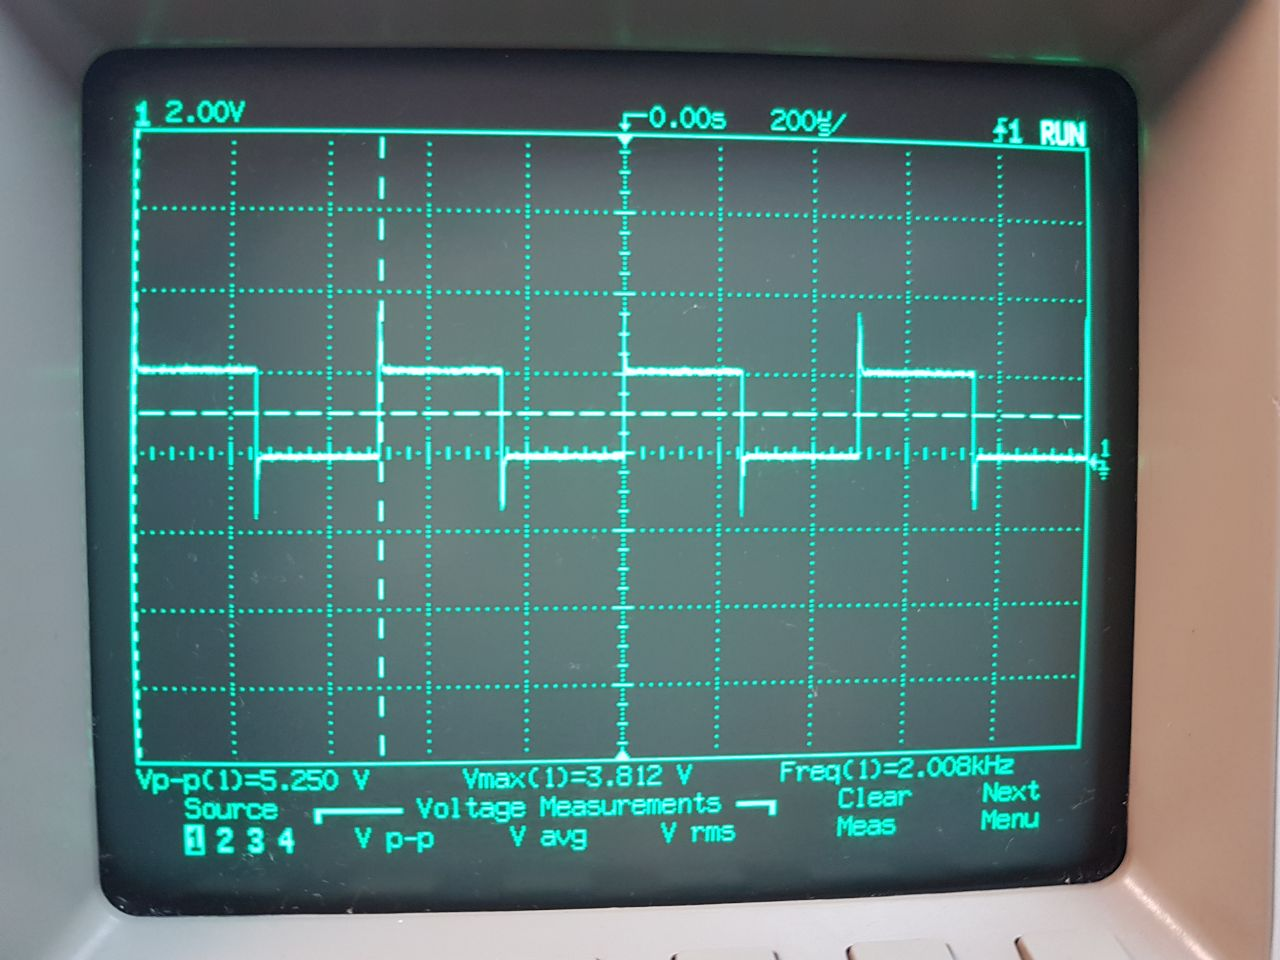
\includegraphics[width=6cm]{1}
		\caption{Respuesta transitoria de Circuito RL.}
	\end{figure}

	Con esto ajustamos la escala del tiempo del osciloscopio para medir el valor de $\tau$ el cual está definido por la siguiente ecuación:
	
	\begin{equation*}
		\tau = \frac{L}{(R_1||R_3)+R_2}
	\end{equation*}
	
	\begin{equation*}
	\tau = \frac{L}{(R_1||R_3)+R_2}
	\end{equation*}
	
	En la imagen se observa el transitorio de la señal y como medimos el valor de $\tau$ ya que sabemos que encontraremos este valor cuando la señal en cuestión llegue al 63\% de su valor nominal.
	
	\begin{figure}[h!]
		\centering
		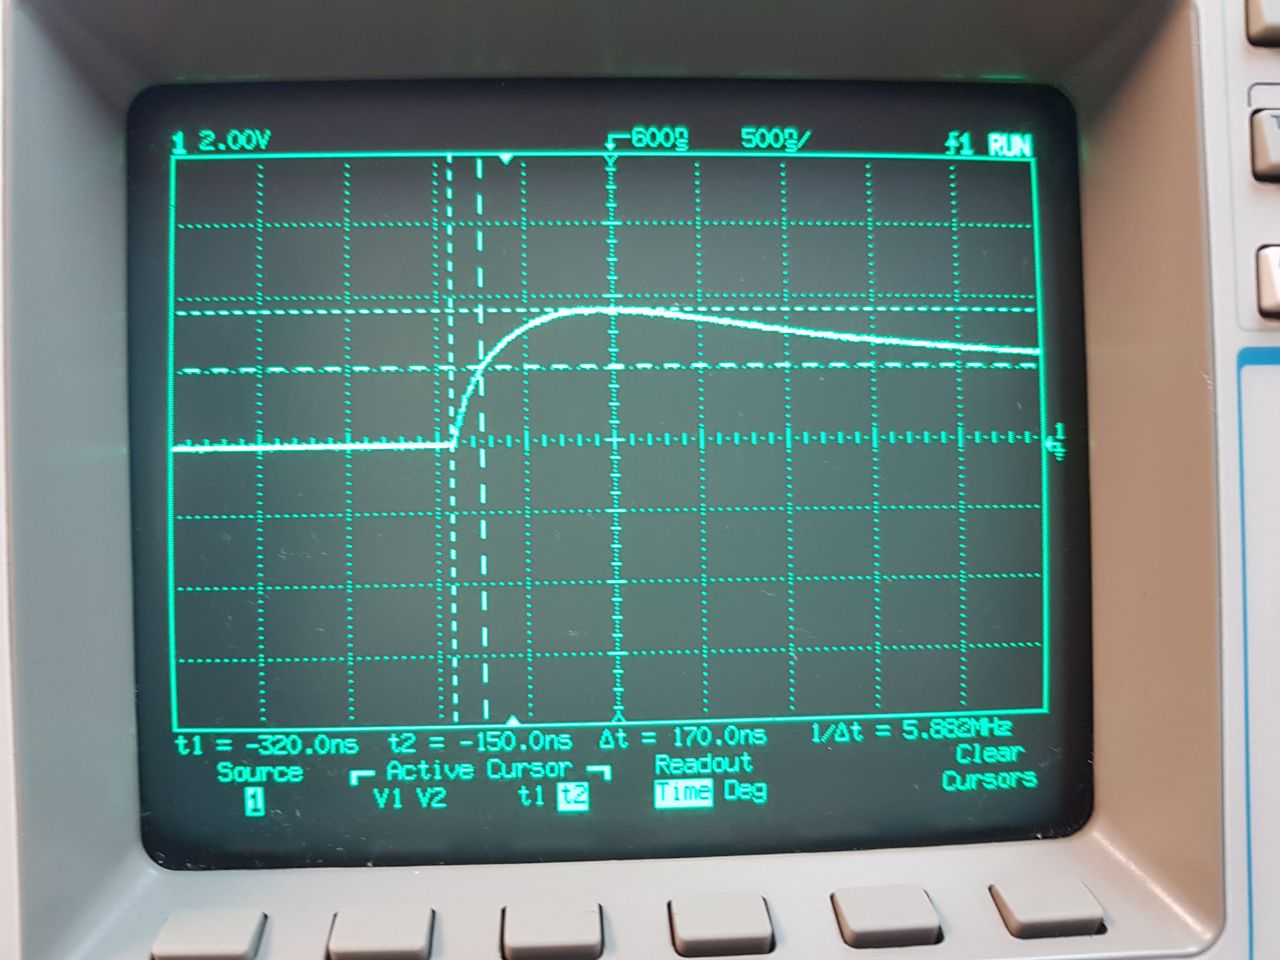
\includegraphics[width=6cm]{2}
		\caption{Medicion de $\tau$ para circuito RL.}
	\end{figure}

	Como podemos observar en la imagen el valor mostrado en el osciloscopio corresponde al valor calculado.
	
	Lo siguiente fue hacer un análisis en CA para ver la respuesta en frecuencia del circuito, en donde se varió la frecuencia en décadas para hacer este barrido de caracterización y se midió el voltaje de salida $V_o$ para un $V_{in}$ de $1V_p$.\\
	\\
	\newpage
	Los resultados fueron los siguientes:
	
	
	\begin{table}[h!]
		\begin{center}
			\begin{tabular}{|c|c||c|c||c|c|}
				\hline	Frecuencia(Hz)	&	Vo(V)	&	Frecuencia(Hz)	&	Vo(V)	&	Frecuencia(Hz)	&	Vo(V)	\\
				\hline	1	&	0.5	&	200	&	0.5	&	30000	&	0.562	\\
				\hline	2	&	0.5	&	300	&	0.5	&	40000	&	0.609	\\
				\hline	3	&	0.5	&	400	&	0.5	&	50000	&	0.64	\\
				\hline	4	&	0.5	&	500	&	0.5	&	60000	&	0.687	\\
				\hline	5	&	0.5	&	600	&	0.5	&	70000	&	0.718	\\
				\hline	6	&	0.5	&	700	&	0.5	&	80000	&	0.75	\\
				\hline	7	&	0.5	&	800	&	0.5	&	90000	&	0.781	\\
				\hline	8	&	0.5	&	900	&	0.5	&	100000	&	0.812	\\
				\hline	9	&	0.5	&	1000	&	0.5	&	200000	&	0.906	\\
				\hline	10	&	0.5	&	2000	&	0.5	&	300000	&	0.89	\\
				\hline	20	&	0.5	&	3000	&	0.5	&	400000	&	0.812	\\
				\hline	30	&	0.5	&	4000	&	0.5	&	500000	&	0.734	\\
				\hline	40	&	0.5	&	5000	&	0.5	&	600000	&	0.671	\\
				\hline	50	&	0.5	&	6000	&	0.5	&	700000	&	0.625	\\
				\hline	60	&	0.5	&	7000	&	0.5	&	800000	&	0.562	\\
				\hline	70	&	0.5	&	8000	&	0.5	&	900000	&	0.546	\\
				\hline	80	&	0.5	&	9000	&	0.5	&	1000000	&	0.5	\\
				\hline	90	&	0.5	&	10000	&	0.5	&		&		\\
				\hline	100	&	0.5	&	20000	&	0.531	&		&		\\
				\hline
			\end{tabular}
			\caption{Barrido en Frecuencia}
		\end{center}
	\end{table}

	Con los resultados obtenidos se construyeron las siguientes graficas:\\
	
	\begin{figure}[h!]
		\centering
		\subfigure[Grafica en V vs Hz]{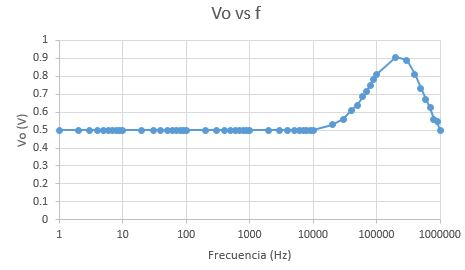
\includegraphics[width=7.5cm]{7}}
		\subfigure[Grafica en dB vs Hz]{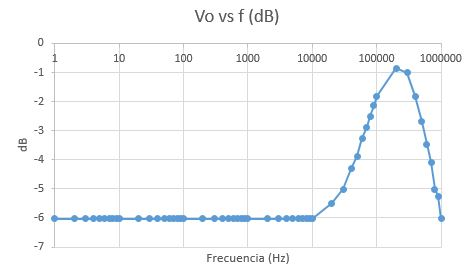
\includegraphics[width=7.5cm]{8}}
		\caption{Grafica de la respuesta en frecuencia.}
	\end{figure}
	
	Por último, se midió la impedancia del inductor a diferentes frecuencias, los resultados son los siguientes:
	
	\begin{figure}[h!]
		\centering
		\subfigure[Impedancia e Inductancia a 100Hz]{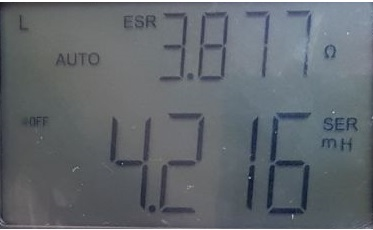
\includegraphics[width=6cm]{4}}
		\subfigure[Impedancia e Inductancia a 120Hz]{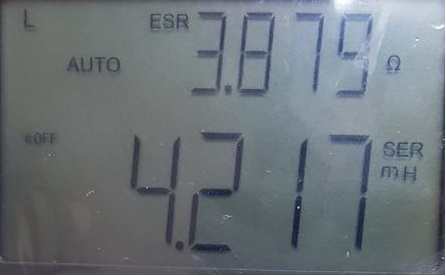
\includegraphics[width=6cm]{3}}
	\end{figure}

	\begin{figure}[h!]
		\centering
		\subfigure[Impedancia e Inductancia a 1kHz]{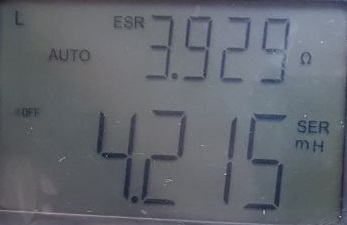
\includegraphics[width=6cm]{5}}
		\subfigure[Impedancia e Inductancia a 10kHz]{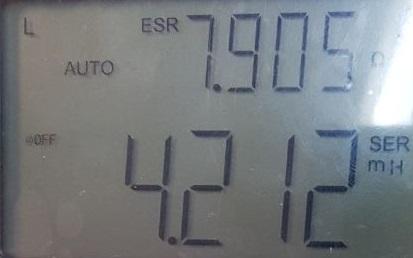
\includegraphics[width=6cm]{6}}
		\caption{Impedancia del inductor a diferentes frecuencias.}
	\end{figure}
%--------------------------------------------------------------------------------------

%Conclusion-------------------------------------------------------------------------------
\newpage
\section{Conclusión de Gerardo Garcia Torres.}
En esta practica se implemento el metodo de obtencion de la funcion de transferencia por inspeccion, el cual resulta un metodo mas practico a diferencia de obtener sus ecuaciones y realizar un análisis del sistema en cuestion.\\[12pt]
Al inicio de la practica se inspecciono una red RC, se obtuvo su funcion de transferencia y su ganancia de DC posteriormente se comprobo con el metodo algebraico y coincidimos en el resultado.\\[12pt]
Al momento de realizar la prueba transitoria (DC) y prueba estacionaria (AC) pudimos observar que la funcion de transferencia nos da informacion del sistema mas aya de la relacion de la señal de salida con la señal de entrada.\\[12pt]
De manera general podemos decir que la funcion de transferencia es un modelo matematico y que ha diversos metodos de obtencion aparte del metodo algebraico
\section{Conclusión de Jose Antonio Andrade Vieyra.}
En esta práctica se pudo observar mejor el como usar la función de transferencia ya que en la práctica anterior no me quedo muy claro del todo. Aparte se pudo observar mejor el comportamiento de los circuitos ya que se simularon en LTspice y me gusto ya que lo que nos dio en la simulación fue lo que nos dio en los resultados prácticos y no se tuvo ningún problema en el laboratorio. Lo que si fue lo más laborioso de obtener fue la función de transferencia por medio del método algebraico ya que no nos daba lo que nos dio con el método de inspección. 
%-----------------------------------------------------------------------------------------

\end{document}